% !TEX root = ../thesis-sample.tex

\chapter{Probabilistic Occupancy Grid Mapping} \label{chap:pogm}

In this chapter, we present the exact solution to occupancy grid map probability for a given depth measurement. This Bayesian approach uses the stochastic properties of sensors, and exploits important patterns in conditional probabilities. Then we show how several measurements can be considered together in 2D. This solution is simulated with numerical examples to show the efficacy of the approach.

\section{Mapping Problem Definition}

Let a map $m$ be decomposed into $n_m$ evenly-spaced grid cells, where the $i$-th grid cell is assigned to a static binary random variable $\mathbf{m}_i$ for $i\in\braces{1,2,\ldots,n_m}$, that is defined as $\mathbf{m}_i=1$ when occupied, and $\mathbf{m}_i=0$ when free. The location and size of each grid cell is assumed known, where a smaller cell size (greater grid resolution) better represents a space, but increases computation and memory. Therefore, a map $m$ is defined by $\{\mathbf{m}_1,\ldots, \mathbf{m}_{n_m}\}$ ($2^{n_{m}}$ possible maps).

Another random variable is defined as $\bar{\mathbf{m}}_i=1-\mathbf{m}_i$ for convenience. The probability that the $i$-th cell is occupied is $P(\mathbf{m}_i)$, and the probability that it is free is $P(\bar{\mathbf{m}}_i)=1-P(\mathbf{m}_i)$. The random variables $\mathbf{m}_i$ are mutually independent, i.e.,
\begin{align}
P(m)=P(\mathbf{m}_1,\mathbf{m}_2,\ldots,\mathbf{m}_{n_m})=\prod_{i=1}^{n_m}P(\mathbf{m}_i).
\end{align}

Consider a range sensor that provides scans of the surrounding environment in order to identify the closest occupied space. The location and the direction of the sensor, referred to as the \emph{pose} at time $t$, is denoted by $X_t=(x_t,R_t)$. In a 2D environment, the planar position and direction of the robot at $t$ are denoted by $x_t\in\Re^2$ and $R_t\in\Sph^1=\braces{q\in\Re^2|\norm{q}=1}$, i.e., the attitude corresponds to a direction on a 2D plane. Similarly in a 3D environment, the spacial position and attitude are denoted by $x_t\in\Re^3$ and $R_t\in\SO=\braces{R\in\Re^{3\times3}|R^\T R=I,\det{R}=1}$. Let $X_{1:t}$ denote the history of poses from the initial time to the current time, i.e., $X_{1:t}=\{X_1,X_2,\ldots, X_t\}$. At each pose, the robot receives a 2D measurement \emph{scan}, composed of $n_z$ measurement \emph{rays}. These rays are 1D depth measurements of known direction from the current pose to the closest occupied space, subject to a known \emph{forward sensor model} $p(z_{t,l}|m,X_t)$, where $z_{t,l}$ is the $l$-th measurement ray of the $t$-th scan $Z_t=\braces{z_{t,1},z_{t,2},\ldots,z_{t,n_z}}$. The measurement history is denoted by $Z_{1:t}=\braces{Z_1,Z_2,\ldots,Z_t}$. 

The probability density function, namely $p(z_{t,l}|m,X_t)$ with respect to the depth of the $l$-th measurement ray conditioned on the map $m$ and the pose $X_t$ is commonly referred to as the \emph{forward sensor model}, which characterizes the corresponding depth sensor, such as the maximum range or accuracy. The forward sensor model satisfies (i) the ranges of all depth measurements are positive and finite, and (ii) a measurement cannot pass through occupied regions. Throughout this paper, we assume that the forward sensor model of the selected sensor is given. This can be determined empirically or analytically. For example, the \emph{beam model for range finders} satisfying  the above criteria is described in~\cite{ThrBurFox05}.

Occupancy grid mapping provides occupancy probabilities based on robot poses and measurement scans. The goal is to obtain $P(\mathbf{m}_i|X_{1:t},Z_{1:t})$, commonly referred to as the \emph{inverse sensor model} for a given forward sensor model $p(z_{t,l}|m,X_t)$ and the initial estimate of the map $P(m)$ with $X_{1:t}$ and $Z_{1:t}$.


\section{Inverse Sensor Model}

In this section, we propose an algorithm to compute the exact inverse sensor model efficiently. 
Suppose the probability of the map conditioned on the past poses and measurements, namely $P(m|X_{1:t-1},Z_{1:t-1})$, is known. Here we construct a posteriori probability $P(m|z_{t,l},X_{1:t},Z_{1:t-1})$, based on the current pose $X_t$, the measurement from the $l$-th ray $z_{t,l}$, and the given forward sensor model $p(z_{t_l}|m,X_t)$.



\subsection{Bayesian Framework}

The occupancy probability $P(m|z_{t,l},X_{1:t},Z_{1:t-1})$ is based on the forward sensor model $p(z_{t,l}|m,X_{1:t},Z_{1:t-1})$ that describe the distribution of the measurements for the given robot pose and the map. This specifies the stochastic characteristics of the sensor are a known distribution, specific to a particular depth sensor. One could certainly obtain a stochastic model by fitting a probability density to a controlled set of measurements. Bayes' rule yields
\begin{align}
\label{eqn:BayesRuleRayISM}
P(&m|z_{t,l},X_{1:t},Z_{1:t-1})%\nonumber\\&
=\frac{p(z_{t,l}|m,X_{1:t},Z_{1:t-1})P(m|X_{1:t-1},Z_{1:t-1})}{p(z_{t,l}|X_{1:t},Z_{1:t-1})},
\end{align}
where the second term in the numerator considers that $X_t$ carries no information about $m$ without $Z_t$.
If the current pose $X_t$ and map $m$ are known, then the measurement ray $z_{t,l}$ is independent of past poses $X_{1:t-1}$ and past measurements $Z_{1:t-1}$ to obtain
\begin{align}
P(m|z_{t,l},&X_{1:t},Z_{1:t-1})%\nonumber\\&
=\eta_{t,l}p(z_{t,l}|m,X_{t})P(m|X_{1:t-1},Z_{1:t-1}),
\end{align}
where the normalizing constant $\eta_{t,l}\in\Re$ absorbs all terms that do not depend on the map $m$.
Next, we compute the occupancy probability of each cell. Let $\mathcal{M}_i$ be the set of maps where the $i$-th cell is occupied, i.e., $\mathcal{M}_i =\{m\in\{0,1\}^{{n_m}}\,|\ \mathbf{m}_i=1\}$. To compute the probability of occupancy of the $i$-th cell, all possible combinations of map in $\mathcal{M}_i$ should be considered, i.e., 
\begin{align}
\label{eqn:InvSenModWithProbDens}
&P(\mathbf{m}_i|z_{t,l},X_{1:t},Z_{1:t-1})%\nonumber\\&
=\eta_{t,l}\sum_{m\in\mathcal{M}_i}p(z_{t,l}|m,X_{t})P(m|X_{1:t-1},Z_{1:t-1}).
\end{align}
Furthermore, to determine the normalizing constant $\eta_{t,l}$, the complement $\\P(\bar{\mathbf{m}}_i|z_{t,l},X_{1:t},Z_{1:t-1})$ must be calculated in the similar manner. Since there are $2^{n_{m}-1}$ maps in $\mathcal{M}_i$, these equations require $2^{n_m}$ terms to compute the summation for the $i$-th grid cell and normalizer, and this process should be repeated for all other cells along the measurement ray. This is the main reason why the existing results are based on approximations or learned solutions of the above expression. 

\subsection{Computationally-Efficient Solution}
% Include Fig 1 from JINT 2017

We propose a computational algorithm to evaluate \refeqn{InvSenModWithProbDens} efficiently~\cite{KauLeeAiMos16,KauTakAiLee17}. 
Since the cells outside of the sensor field of view (FOV) are not affected, we focus on a reduced map $r_l$ in the FOV of the $l$-th ray. This reduced map is chosen such that each cell of $r_l$ corresponds to a grid cell of map $m$ that the $l$-th ray intersects, ordered by increasing distance. Let $\mathbf{r}_{l,k}$ be the binary random variable representing the occupancy of the $k$-th cell of the $l$-th ray. The number of cells in the reduced map is denoted by $n_{r,l}\leq n_m$.

Next, let $\mathbf{r}_{l,k+}$ correspond to the event that the $k$-th cell of the $l$-th ray is occupied, cells with lower index (closer cells) are free, and cells with greater index (farther cells) may or may not be occupied, i.e., event $\mathbf{r}_{l,k+}$ occurs when \\$r\in\braces{r\in\{0,1\}^{{n_{r,l}}}\,|\mathbf{r}_{l,1}=0,\mathbf{r}_{l,2}=0,\ldots,\mathbf{r}_{l,k-1}=0,\mathbf{r}_{l,k}=1}$. Put differently, the $k$-th cell $\mathbf{r}_{l,k}$ is the closest occupied cell to current pose $X_t$ along the $l$-th ray. For example, see Figure \ref{fig:show_rkplus} that illustrates the event of $\mathbf{r}_{l,k+}$ when $l=1$ and $k=4$ for an one-dimensional cell array. This concept of grouping map outcomes can be easily extended to 2D using ray casting, where a 1D ray is spanning 2D space, which is easily determined from geometry, described in further detail in Section \ref{sec:RayCasting}. Then, the forward sensor model is identical for all maps defined by $\mathbf{r}_{l,k+}$, regardless of the occupancy of the cells beyond the $k$-th cell, and the corresponding forward sensor model $p(z_{t,l}|\mathbf{r}_{l,k+},X_{t})$ depends on the distance from $X_t$ to the $k$-th cell. Based on this, we present the mathematical expressions for the exact inverse sensor model, as summarized by \refeqn{RayISMAnswer} in Proposition \ref{prop:ISM}. Later in Section \ref{sec:RayScanComb}, these are also rearranged in computational algorithms. 



\begin{figure}
  \centering
  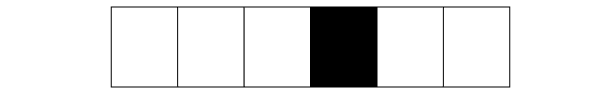
\includegraphics[width=0.4\textwidth]{rkplus_1.png}
    \centering
  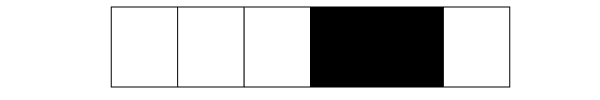
\includegraphics[width=0.4\textwidth]{rkplus_2.png}  
  \centering
  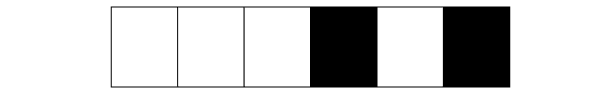
\includegraphics[width=0.4\textwidth]{rkplus_3.png}
    \centering
  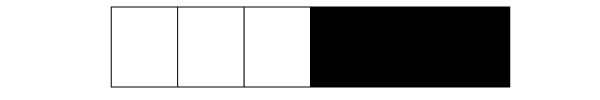
\includegraphics[width=0.4\textwidth]{rkplus_4.png}
  \caption{Occupancy Grid Maps with Identical Forward Sensor Models}
  \medskip
  \small
  A robot located to the left of a 1D occupancy grid map $r_l$ composed of $n_{r,l}=6$ grid cells in four cases. In each case, cells the first three cells are free, the fourth cell is occupied, and the fifth and sixth cells may or may not be occupied. All above outcomes correspond to the event $\mathbf{r}_{l,4+}$.
  \label{fig:show_rkplus}
\end{figure}

\begin{prop}
\label{prop:ISM}
For the $l$-th measurement ray, the a posteriori probability of the occupancy of the $k$-th cell, namely the ray inverse sensor model, is given by
\begin{align}
\label{eqn:RayISMAnswer}
P(\mathbf{r}_{l,k}|z_{t,l},X_{1:t},Z_{1:t-1})&=\eta_{t,l}\tilde P(\mathbf{r}_{l,k}|z_{t,l},X_{1:t},Z_{1:t-1}),
\end{align}
where the unnormalized probability of the inverse sensor model is defined as
\begin{align}
\label{eqn:Unnormalized}
& \tilde P(\mathbf{r}_{l,k}|z_{t,l},X_{1:t},Z_{1:t-1})%\nonumber\\&
=P(\mathbf{r}_{l,k}|X_{1:t-1},Z_{1:t-1})\nonumber\\
&\quad\times 
\bigg[\sum_{i=1}^{k-1}\bigg\{\prod_{j=0}^{i-1}P(\bar{\mathbf{r}}_{l,j}|X_{1:t-1},Z_{1:t-1})\bigg\}%\nonumber\\
%&\quad\times 
p(z_{t,l}|\mathbf{r}_{l,i+},X_t)P(\mathbf{r}_{l,i}|X_{1:t-1},Z_{1:t-1})\bigg]\nonumber\\
&\quad + \bigg\{\prod_{j=0}^{k-1}P(\bar{\mathbf{r}}_{l,j}|X_{1:t-1},Z_{1:t-1})\bigg\}%\nonumber\\
%&\quad\times 
p(z_{t,l}|\mathbf{r}_{l,k+},X_t)P(\mathbf{r}_{l,k}|X_{1:t-1},Z_{1:t-1}),
\end{align}
where $P(\bar{\mathbf{r}}_{l,0}|X_{1:t-1},Z_{1:t-1})=P(\mathbf{r}_{l,n_r+1}|X_{1:t-1},Z_{1:t-1})=1$ is chosen for convenience and $p(z_{t,l}|\mathbf{r}_{l,(n_r+1)+},X_t)$ represents the probability density of the measurement when all of cells in the field of view of the $l$-th ray is not occupied. The normalizer $\eta_{t,l}$ is given by
\begin{align}
\label{eqn:allEta}
\eta_{t,l}
&=
\bigg[\sum_{i=1}^{n_{r,l}+1}\bigg\{\prod_{j=0}^{i-1}P(\bar{\mathbf{r}}_{l,j}|X_{1:t-1},Z_{1:t-1})\bigg\}p(z_{t,l}|\mathbf{r}_{l,i+},X_t)P(\mathbf{r}_{l,i}|X_{1:t-1},Z_{1:t-1})\bigg]^{-1},
\end{align}
and it is independent of the cell index $k$.
\end{prop}
\begin{proof}% TODO: add ref?
See Appendix A.
\end{proof}

%Note that the a priori estimate, $P(\mathbf{r}_{l,k}|X_{1:t-1},Z_{1:t-1})$ and its compliment $\\P(\bar{\mathbf{r}}_{l,k}|X_{1:t-1},Z_{1:t-1})=1-P(\mathbf{r}_{l,k}|X_{1:t-1},Z_{1:t-1})$ are available at the $t$-th step. Then, \refeqn{RayISMAnswer} yields a sequential occupancy grid mapping that can be applied whenever new measurements are available. 

%where a priori probability is $\mathbf{P}_k^-=P(\mathbf{r}_{k}|X_{1:t-1},Z_{1:t-1})$, its complement is $\bar{\mathbf{P}}_k^-=1-\mathbf{P}_k^-$, $P(\bar{\mathbf{r}}_{0}|X_{1:t-1},Z_{1:t-1})=P(\mathbf{r}_{n_{r,l}+1}|X_{1:t-1},Z_{1:t-1})=1$ for convenience, and $p(z_{t,l}|\mathbf{r}_{(n_{r,l}+1)+},X_t)$ represents the forward sensor model of a maximum sensor reading. 
%The proofs of \refeqn{RayISMAnswer}--\refeqn{Unnormalized} are given in~\cite{KauLeeAiMos16}. 

Since $\tilde P(\mathbf{r}_{l,k}|z_{t,l},X_{1:t},Z_{1:t-1})$ from \refeqn{Unnormalized} uses several repeated terms from the prior $\tilde P(\mathbf{r}_{l,k-1}|z_{t,l},X_{1:t},Z_{1:t-1})$, and $\eta_{t,l}$ is easily obtained from these as well, the computational cost of \refeqn{RayISMAnswer} is linear with respect to the number of cells along a measurement ray, amortized to $\mathcal{O}(1)$ for each cell. Because of this substantial computational improvement, the exact inverse sensor model can be applied in real-time. The process of updating each cell along a measurement ray is repeated for all rays composing scan $Z_t$.

% TODO: add update paragraph from JINT18

%Compared with \refeqn{InvSenModWithProbDens}, where the terms of the summation should be repeated $2^{n_{r,l}}$ times \emph{per each cell of the reduced map}, the proposed expressions \refeqn{RayISMAnswer} and \refeqn{allEta} are \textit{substantially} simpler. In fact, if \refeqn{Unnormalized} and \refeqn{allEta} are obtained recursively, requiring the summation of $O(n_{r,l}+1)$ rather than $O(n_{r,l}\times2^{n_{r,l}})$ as previously thought for \emph{all cells of the reduced map}, this yields an algorithm that is $\mathbf{n_{r,l}\times2^{n_{r,l}}/(n_{r,l}+1)}$ \textbf{times faster}.

\section{Mapping in 2D Space}

The above formulations describe how a single ray updates grid cells along its 1D path. Next we describe how measurement rays can update 2D maps, and how large scans of measurement rays are handled together.

% show RayCastingIllustration.png
\subsection{Ray Casting}
\label{sec:RayCasting}

Ray casting is the process of determining which cells a measurement ray might intersect, and the distances to these cells. The process is straightforward: follow a measurement unit vector from its minimum range $z_\text{min}$ to maximum range $z_\text{max}$, and identify the edges of all grid cells that it intersects. Save the cell index and Cartesian distance from the robot, and re-order the cells by increasing distance. An illustration of a simple example is shown in Figure \ref{fig:RayCastingIllustration}.

\begin{figure}[!ht]
    \centering
    \begin{subfigure}[t]{0.4\columnwidth}
        \centering
        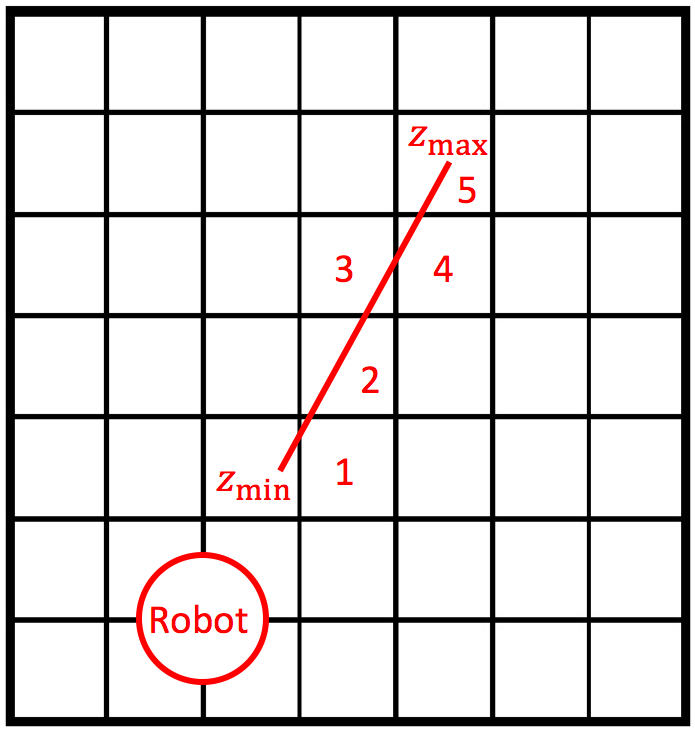
\includegraphics[width=\textwidth]{RayCastingIllustration.png}
        \caption{Ray Casting on a 2D Grid}
%        \label{fig:penn_map_total}
    \end{subfigure}
    \hspace*{0.05\columnwidth}
    \begin{subfigure}[t]{0.4\columnwidth}
        \centering
        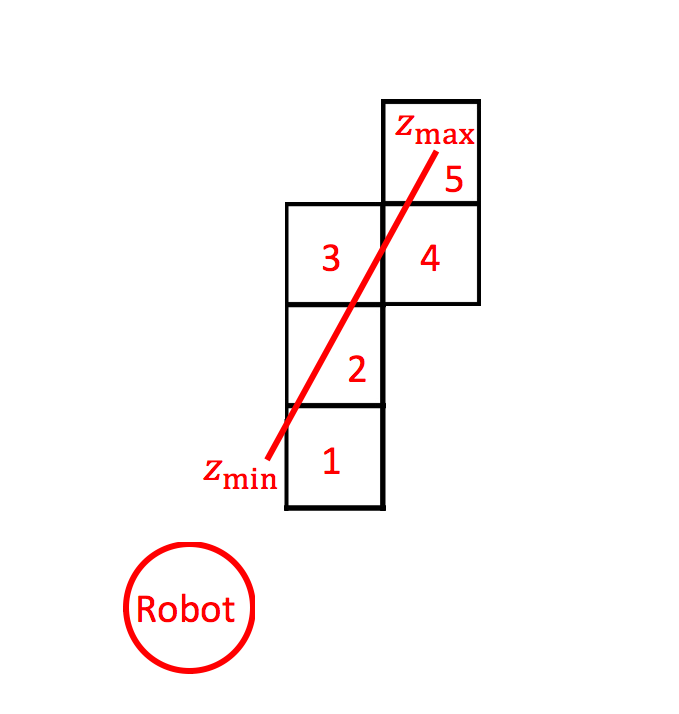
\includegraphics[width=\textwidth]{RayCastIllustrationReducedMapOnly.png}
        \caption{Reduced Map Only}
%        \label{fig:penn_map_zoom}
    \end{subfigure}
    \caption{Ray Casting Illustration}
    \label{fig:RayCastingIllustration}
    	\medskip
  	\small
	This simple 2D example illustrates how ray casting determines the cells that compose the reduced map for the inverse sensor model. The closest edges are used to determine which cells should be considered, and in what order. The complete map cell indices are temporarily saved as well, which are used to associate probabilities to cells of the reduced map.
\end{figure}

\subsection{Combining Measurements from a Single Scan}
\label{sec:RayScanComb}
Typically, many measurement rays are provided from a single scan from modern sensors.
Next, we describe two approaches to combine the inverse sensor models of numerous measurement rays.

\paragraph{Ray-By-Ray Approach}

At the $t$-th time step, consider the measurement scan $Z_t=\{z_{t,1},z_{t,2},...,z_{t,n_z}\}$. One may apply the results of Proposition \ref{prop:ISM} repeatedly for each ray to obtain a two-dimensional inverse sensor model because
\begin{align}
\label{eqn:RayByRayScanISM}
P(\mathbf{m}_i|X_{1:t},Z_{1:t})&%=P(\mathbf{m}_i|X_{1:t},Z_{1:t-1}|z_{t,1},z_{t,2},...,z_{t,n_z})\nonumber\\&
=P(\mathbf{m}_i|X_{1:t},Z_{1:t-1}|z_{t,1}|z_{t,2}|...|z_{t,n_z}).
\end{align}
In this approach, each ray is considered individually such that the inverse sensor model updates the probabilities of grid cells from one ray before subsequent rays of $Z_t$ are considered. Therefore, we assume the first measurement ray $z_{t,1}$ is independent of the remaining rays $z_{t,2:n_z}$. For the second ray, namely $z_{t,2}$, this may depend on $z_{t,1}$, but not subsequent rays $z_{t,3:n_z}$. By the time $z_{t,n_z}$ is considered, it may depend on all prior rays $z_{t,1:n_z-1}$. Therefore, the ray-by-ray approach considers rays within a single scan as partially dependent on each other.

In short, the proposed scan inverse sensor model is computed by \refeqn{RayISMAnswer}-\refeqn{RayByRayScanISM}. These are summarized in Algorithm \ref{alg:RayByRayISM} as a computationally efficient, recursive algorithm that avoids several repeated calculations of the same quantity. This algorithm utilizes temporary variables, where the required computational resources are minimized by computing the updated occupancy probabilities of all grid cells along a measurement ray together. Note that this function is only considering $l$-th ray at the $t$-th time step, where probabilities are subject to conditions on the history of poses $X_{1:t-1}$ and measurement scans $Z_{1:t-1}$, so these are removed from the algorithm for simplicity.

\vspace*{0.05\columnwidth}
\begin{algorithm}[H]
	Function: $P(m|X,Z)=\text{InverseSensorModelRayByRay}(P(m),X,Z)$\;
	% $\forall$ $l\in\braces{1,2,\ldots,n_{l}}$\;
	
	\For{$l=1,2,\ldots,n_{l}$}{
		Find $n_{r,l}$ cells from $m$ corresponding to $z_l$\;
		Initialize $\eta_l^{-1}=0$ and $P(\bar{\mathbf{r}}_{l,0}|X,z_{1:l-1})=1$ ($z_{1:0}$ is no condition)\;
		\For{$k=1,2,\ldots,n_{r,l}$}{
			$P(\mathbf{r}_{l,k+}|X,z_{1:l-1}) = P(\bar{\mathbf{r}}_{l,0:k-1}|X,z_{1:l-1})P(\mathbf{r}_{l,k}|X,z_{1:l-1})$\;
			$P(\bar{\mathbf{r}}_{l,0:k}|X,z_{1:l-1})=P(\bar{\mathbf{r}}_{l,0:k-1}|X,z_{1:l-1})(1-P(\mathbf{r}_{l,k}|X,z_{1:l-1}))$\;
    			$a_\text{temp}=P(\mathbf{r}_{l,k+}|X,z_{1:l-1})p(z_l|\mathbf{r}_{1:l,k+},X)$\;
   			$\tilde P(\mathbf{r}_{l,k}|X,z_{1:l})=P(\mathbf{r}_{l,k}|X,z_{1:l-1})\eta^{-1}_{l}+a_\text{temp}$\;
   			$\eta_l^{-1}=\eta_l^{-1}+a_\text{temp}$\;
		}
	$\eta_l^{-1}=\eta_l^{-1}+P(\bar{\mathbf{r}}_{l,0:n_{r,l}}|X,z_{1:l-1})p(z_\text{max})$\;
	$P(\mathbf{r}_{k}|z_{1:l})=\eta_l\tilde P(\mathbf{r}_{k}|X,z_{1:l})$ for all $k\in\braces{1,2,\ldots,n_{r,l}}$\;
	Substitute $P(\mathbf{r}_{k}|X,z_{1:l})$ back into $P(m|X,z_{1:l})$\;
	}
	Return $P(m|X,z_{1:n_{l}})=P(m|X,Z)$\;
\caption{Inverse Sensor Model of a Scan Updated Ray-By-Ray}
\label{alg:RayByRayISM}
\end{algorithm}
\vspace*{0.05\columnwidth}
\newpage





\paragraph{Synergistic Update Approach}

In this approach, all rays from a single scan are considered simultaneously for a synergistic update of all grid cells falling inside the scan FOV. However, the subsequent formulations require the assumption that all measurement rays within the scan are mutually independent, i.e.,
\begin{align*}
p(z_{t,1},z_{t,2},\ldots,z_{t,n_l}|\mathbf{m}_i,X_{1:t},Z_{1:t-1})=\prod_{l=1}^{n_l}p(z_{t,l}|\mathbf{m}_i,X_{1:t},Z_{1:t-1}).
\end{align*}
Here, we construct such two-dimensional inverse sensor model, referred to as the synergistic scan inverse sensor model.
Let $\mathcal L_i\subset\{1,\ldots, n_l\}$ be the set of rays that pass through the $i$-th cell, $\mathbf{m}_i$. Applying Bayes' rule repeatedly, we obtain
\begin{align}
P(\mathbf{m}_i|X_{1:t},Z_{1:t})
&=\tilde\zeta_i\braces{\prod_{l\in\mathcal{L}_i}p(z_{t,l}|\mathbf{m}_i,X_{1:t},Z_{1:t-1})}P(\mathbf{m}_i|X_{1:t-1},Z_{1:t-1})\nonumber\\
&=
\zeta_i P(\mathbf{m}_i|X_{1:t-1},Z_{1:t-1})%\nonumber\\&\quad\times
\prod_{l\in\mathcal{L}_i}\frac{P(\mathbf{m}_i|z_{t,l},X_{1:t},Z_{1:t-1})}{P(\mathbf{m}_i|X_{1:t-1},Z_{1:t-1})},
\label{eqn:ThirdBayesRule}
\end{align}
where $\tilde\zeta_i,\zeta_i\in\Re$ correspond to normalizing constants independent of $\mathbf{m}_i$. 

Suppose the $l$-th measurement ray intersects with the cell $\mathbf{m}_i$, and it is the $k$-th cell of the corresponding reduced map, i.e., $\mathbf{r}_{l,k}$ corresponds to the cell $\mathbf{m}_i$ in the $l$-th reduced map, and $\mathbf{r}_{l,k}=\mathbf{m}_i$ since they represent the same cell.  Then, we have $P(\mathbf{m}_i|z_{t,l},X_{1:t},Z_{1:t-1})=P(\mathbf{r}_{l,k}|z_{t,l},X_{1:t},Z_{1:t-1})=\eta_{t,l}\tilde P(\mathbf{r}_{l,k}|z_{t,l},X_{1:t},Z_{1:t-1})$. 

\sloppy Using this, \refeqn{ThirdBayesRule} is rewritten as
\begin{align}
P(\mathbf{m}_i|X_{1:t},Z_{1:t})
&=\xi_i P(\mathbf{m}_i|{X_{1:t-1}},Z_{1:t-1})
\prod_{l\in\mathcal L_i}
\hat P(\mathbf{r}_{l,k}|z_{t,l},X_{1:t},Z_{1:t-1})
,
\label{eqn:ISM_Fusion}
\end{align}
where the normalizer $\xi_i$ is composed of the product of normalizers $\zeta_i$, and $\eta_i$. Here, we introduce a new term $\hat P(\mathbf{r}_{l,k}|z_{t,l},X_{1:t},Z_{1:t-1})$ for computational efficiency as
\begin{align}
&\hat P(\mathbf{r}_{l,k}|z_{t,l},X_{1:t},Z_{1:t-1})
\triangleq \frac{\tilde P(\mathbf{r}_{l,k}|z_{t,l},X_{1:t},Z_{1:t-1})}{P(\mathbf{m}_i|X_{1:t-1},Z_{1:t-1})}
\nonumber\\&=
\sum_{i=1}^{k-1}\bigg\{\prod_{j=0}^{i-1}P(\bar{\mathbf{r}}_{l,j}|X_{1:t-1},Z_{1:t-1})\bigg\}p(z_{t,l}|\mathbf{r}_{l,i+},X_t)P(\mathbf{r}_{l,i}|X_{1:t-1},Z_{1:t-1})
\nonumber\\&\quad
+
\bigg\{\prod_{j=0}^{k-1}P(\bar{\mathbf{r}}_{l,j}|X_{1:t-1},Z_{1:t-1})\bigg\}p(z_{t,l}|\mathbf{r}_{l,k+},X_t),
\end{align}
where we have used \refeqn{Unnormalized}. Similarly, its complement is
\begin{align}
P(\bar{\mathbf{m}}_i|{{X_{1:t}}},Z_{1:t})
&=\xi_i P(\bar{\mathbf{m}}_i|{X_{1:t-1}},Z_{1:t-1})
\prod_{l\in\mathcal L_i}
\hat P(\bar{\mathbf{r}}_{l,k}|z_{t,l},X_{1:t},Z_{1:t-1})
,
\label{eqn:ISM_Bar_Fusion}
\end{align}
where $\hat P(\bar{\mathbf{r}}_{l,k}|z_{t,l},X_{1:t},Z_{1:t-1})$ is defined as
\begin{align}
&\hat P(\bar{\mathbf{r}}_{l,k}|z_{t,l},X_{1:t},Z_{1:t-1})
\triangleq\frac{\tilde P(\bar{\mathbf{r}}_{l,k}|z_{t,l},X_{1:t},Z_{1:t-1})}{P(\bar{\mathbf{m}}_i|X_{1:t},Z_{1:t-1})}
\nonumber\\
&=\sum_{i=1}^{k-1}\bigg\{\prod_{j=0}^{i-1}P(\bar{\mathbf{r}}_{l,j}|X_{1:t-1},Z_{1:t-1})\bigg\} p(z_{t,l}|\mathbf{r}_{l,i+},X_t)P(\mathbf{r}_{l,i}|X_{1:t-1},Z_{1:t-1})
\nonumber
\\
&\quad
+\frac{
\sum_{i=k+1}^{n_{r,l}+1}\bigg\{\prod_{j=0}^{i-1}P(\bar{\mathbf{r}}_{l,j}|X_{1:t-1},Z_{1:t-1})\bigg\}p(z_{t,l}|\mathbf{r}_{l,i+},X_t)P(\mathbf{r}_{l,i}|X_{1:t-1},Z_{1:t-1})}{P(\bar{\mathbf{r}}_{l,k}|X_{1:t-1},Z_{1:t-1})},
\end{align}
which is obtained from \refeqn{tildePbar}. Since % TODO: ref in appendix
\begin{align*}
P(\mathbf{m}_i|X_{1:t},Z_{1:t})+P(\bar{\mathbf{m}}_i|X_{1:t},Z_{1:t})=1,
\end{align*}
the normalizer $\xi_i$ is obtained using \refeqn{ISM_Fusion} and \refeqn{ISM_Bar_Fusion} as,
\begin{align}
&\xi_i=
\bigg[
P(\mathbf{m}_i|{X_{1:t-1}},Z_{1:t-1})
\prod_{\mathcal L_i}
\hat P(\mathbf{r}_{l,k}|z_{t,l},{X_{1:t}},Z_{1:t-1})
\nonumber\\&\quad
+
P(\bar{\mathbf{m}}_i|{X_{1:t-1}},Z_{1:t-1})
\prod_{\mathcal L_i}
\hat P(\bar{\mathbf{r}}_{l,k}|z_{t,l},X_{1:t},Z_{1:t-1})
\bigg]^{-1},\label{eqn:xi}
\end{align}
which is substituted into \refeqn{ISM_Fusion} to obtain the complete scan inverse sensor model $P(\mathbf{m}_i|X_{1:t},Z_{1:t})$. 


The synergistic scan inverse sensor model algorithm is summarized with the pseudo-code of Algorithm \ref{alg:SynergisticScanISM} as a computationally efficient, recursive algorithm that avoids repeated calculations of the same quantity. This algorithm utilizes the following temporary variables to develop the algorithm in an efficient recursive form, defined as
\begin{align*}
a_k&=\sum_{i=1}^{k-1}\bigg\{\prod_{j=0}^{i-1}P(\bar{\mathbf{r}}_{l,j}|X_{1:t-1},Z_{1:t-1})\bigg\}p(z_{t,l}|\mathbf{r}_{l,i},X_t)P(\mathbf{r}_{l,i}|X_{1:t-1},Z_{1:t-1}),
\\
b_k&=\prod_{j=0}^{k-1}P(\bar{\mathbf{r}}_{l,j}|X_{1:t-1},Z_{1:t-1}),
\nonumber\\
c_k&=\frac{
\sum_{i=k+1}^{n_{r,l}+1}\bigg\{\prod_{j=0}^{i-1}P(\bar{\mathbf{r}}_{l,j}|X_{1:t-1},Z_{1:t-1})\bigg\}p(z_{t,l}|\mathbf{r}_{l,i+},X_t)P(\mathbf{r}_{l,i}|X_{1:t-1},Z_{1:t-1})}{P(\bar{\mathbf{r}}_{l,k}|X_{1:t-1},Z_{1:t-1})},
\end{align*}
as well as $d$ and $e$ for the two terms composing \refeqn{xi}. Once again, the history of poses and measurement scans are removed from the pseudo-code for simplicity.

% TODO: check spacing of algorithms once complete
\vspace*{0.05\columnwidth}
\begin{algorithm}[H]
	Function: $P(m|X,Z)=\text{InverseSensorModelSynergistic}(P(m),X,Z)$\;
	\For{$l=1,2,\ldots,n_{l}$}{
		Find $n_{r,l}$ cells from $m$ corresponding to $z_l$\;
		Define $P(\mathbf{r}_{l,0})=0$, $P(\bar{\mathbf{r}}_{l,0})=1$, $P(\mathbf{r}_{l,n_{r,l}+1})=1$, and $c_{n_{r,l}+1}=0$\;
		\For{$k=1,2,\ldots,n_{r,l}$}{
			\If{$k=1$}{
				$a_1=0$, $b_1=1$\;
			}
			\Else{
				$a_k=a_{k-1}+b_{k-1}p(z_{l}|\mathbf{r}_{l,k-1},X)P(\mathbf{r}_{l,k-1})$, $b_k=b_{k-1}P(\bar{\mathbf{r}}_{l,k-1})$\;
			}
		}
		\For{$k = n_{r,l},n_{r,l}-1,...,1$}{
			$c_k=\frac{P(\mathbf{r}_{l,k+1})}{P(\bar{\mathbf{r}}_{l,k})}c_{k+1}+b_{k}p(z_{t,l}|\mathbf{r}_{l,k+1},X)P(\mathbf{r}_{l,k+1})$\;
		}
		\For{$k = 1,2,...,n_{r,l}$}{
			$\hat P(\mathbf{r}_{l,k}|z_{t,l},X)=a_k+b_kp(z_{t,l}|\mathbf{r}_{l,k},X)$, $\hat P(\bar{\mathbf{r}}_{l,k}|z_{t,l},X,)=a_k+c_k$\;
		}
	}
	\For{$i\in m_\text{FOV}$ \text{(map cells inside FOV)}}{
		Obtain the set $\mathcal L_i$ of $l_i$ measurement rays intersecting this cell\;
		\If{$l_i>0$}{
			$d=P(\mathbf{m}_i)\prod_{\mathcal L_i}\hat P(\mathbf{r}_{l,k}|z_{t,l},X)$\;
			$e=P(\bar{\mathbf{m}}_i)\prod_{\mathcal L_i}\hat P(\bar{\mathbf{r}}_{l,k}|z_{t,l},X)$\;
			$P(\mathbf{m}_i|X,Z)=\frac{d}{d+e}$\;
		}
		\Else{
			$P(\mathbf{m}_i|X,Z)=P(\mathbf{m}_i)$\;
		}
	}
	Return $P(m|X,Z)$\;
\caption{Inverse Sensor Model of a Scan Updated Synergistically}
\label{alg:SynergisticScanISM}
\end{algorithm}
\vspace*{0.05\columnwidth}



In short, we propose two alternatives for combining inverse sensor models for multiple rays within a scan. The ray-by-ray approach updates the entire map one ray at a time with some dependencies among the rays, while the synergistic approach considers all rays together where rays are assumed mutually independent.

% TODO: move to 3D mapping part
%\subsection{Multi-Sensor Fusion}

% TODO: move to experiment part
%\subsection{Practical Implications}

\subsection{Numerical Examples}

In contrast to the current approximate inverse sensor models, the proposed ray-by-ray and synergistic algorithms evaluate the exact inverse sensor model efficiently without relying on approximations, learned solutions, or log-odds ratio assumptions. The following simulations show two examples comparing an approximate inverse sensor model with the proposed exact inverse sensor model, either with integrating multiple measurements ray-by-ray or synergistically. The proposed algorithms yield substantially more accurate maps for the same set of measurements.


\paragraph{Approximate Inverse Sensor Model}

We compare the proposed exact solution to the inverse sensor model with an approximate algorithm developed for a Microsoft Kinect sensor~\cite{PirRutBisSch11,KhoElb12}, summarized as follows. The probability that the $i$-th grid cell $\mathbf{m}_i$ is occupied conditioned on the measurement ray $z_{t,l}$ (the $l$-th ray at the $t$-th time step) at the pose $X_t$ is the continuous function
\begin{align}
\label{eqn:ISM_Approx_1}
P(\mathbf{m}_i|z_{t,l},X_t)=\begin{cases}
0.3+(\frac{k}{\sigma\sqrt{2\pi}}+0.2)e^{-\frac12\left(\frac{\hat z_{l,i}-z_{t,l}}{\sigma}\right)^2}\ &\text{if}\ z_{t,l}\leq \hat z_{l,i},
\\
0.5+\frac{k}{\sigma\sqrt{2\pi}}e^{-\frac12\left(\frac{\hat z_{l,i}-z_{t,l}}{\sigma}\right)^2}\ &\text{if}\ z_{t,l}>\hat z_{l,i},
\end{cases}
\end{align}
which is based on the expected distance to the cell $\hat z_{l,i}$ with parameters $k=\sigma=0.6$. This follows the structure of the approximate inverse sensor model proposed in~\cite{Andert09}. The main idea of this approach is that the probability of a cell being occupied (i) near a measurement is high (measurement likely hits this cell), (ii) between the robot and the measurement is low (measurement passes through these cells), and (iii) beyond the measurement is unchanged (the robot cannot measure through a wall/object). 

Then, these probabilities are combined in a weighted fashion such that all measurements rays of scan $Z_t$ simultaneously update the same grid cell in a log-odds format,
\begin{align}
\label{eqn:ISM_Approx_2}
\log\left(\frac{P(\mathbf{m}_i|Z_{t},X_t)}{1-P(\mathbf{m}_i|Z_{t},X_t)}\right)
=
\frac1{\sum_{z_{t,l}\in\mathbf{m}_i}\hat z_{l,i}}\sum_{z_{t,l}\in\mathbf{m}_i}\log\left(\frac{P(\mathbf{m}_i|z_{t,l},X_t)}{1-P(\mathbf{m}_i|z_{t,l},X_t)}\hat z_{l,i}\right).
\end{align}


\paragraph{Mapping a Hallway with the Ray-By-Ray Approach}

First, we compare the proposed exact solution to the ray-by-ray inverse sensor model summarized in Algorithm \ref{alg:RayByRayISM} with an approximations of \refeqn{ISM_Approx_1}--\refeqn{ISM_Approx_2}.
Table~\ref{tab:penn} shows the mapping parameters and data specifications for the actual odometry and lidar measurements from University of Pennsylvania through Coursera open course~\cite{coursera}. Among these parameters, cell resolution and the number of rays have the greatest impact on computation. In general, the finer the grid, the greater the memory and computational requirements are because the computational order of \refeqn{RayISMAnswer} grows linearly with the number of grid cells inside the sensor range limits. Since the inverse sensor models are combined sequentially as shown in \refeqn{RayByRayScanISM}, the number of rays considered are proportional to the computation order as well.
Figure~\ref{fig:penn_map} shows the direct comparison of the resulting map based on the approximate and proposed inverse sensor model.
As shown in the figure, both approaches capture the structure of the environment. However, the significant differences can be seen, particularly with an enlarged mapping section in Figure~\ref{fig:penn_map_zoom}.

To quantify the degree of map uncertainty, we define the entropy of the map as 
\begin{align*}
H(P(m|X_{1:t},Z_{1:t}))&=-\sum_{i=1}^n\big\{P(\mathbf{m}_i|X_{1:t},Z_{1:t})\log P(\mathbf{m}_i|X_{1:t},Z_{1:t})\nonumber\\
&\qquad+(1-P(\mathbf{m}_i|X_{1:t},Z_{1:t}))\log(1-P(\mathbf{m}_i|X_{1:t},Z_{1:t}))\big\},
\end{align*}
which is maximized when the probability of occupancy is $0.5$ for all cells (more uncertain), and it is minimized when they are either $0$ or $1$ (less uncertain). 
The entropy differences among the algorithms can be clearly depicted in Figure~\ref{fig:entropy_comp} at frame 2280.
The red part of the map shows the maximum  entropy whereas blue shows lowest entropy for the cell.
Finally, overall improvement was demonstrated in Figure~\ref{fig:entropy} resulting in an improved entropy value per grid cell throughout the mapping process.
In short, the proposed exact occupancy grid mapping produced a cleaner map with lower entropy from the same set of measurements.

\begin{center}
\captionof{table}{Experimental Parameters Provided from the Dataset}
\label{tab:penn}
    \begin{tabular}{r | c}
        Parameters & Value\\ \hline\hline
        Map dimension & 576x448 [pixel]\\
        Resolution & 1/16 [m]\\
        Scan angle & [-2.36, 2.36]\\
        Ray number & 1081\\
        Total frame & Every 120 scans out of 3701\\
    \end{tabular}
\end{center}

\begin{figure}[!ht]
    \centering
    \begin{subfigure}[t]{0.8\columnwidth}
        \centering
        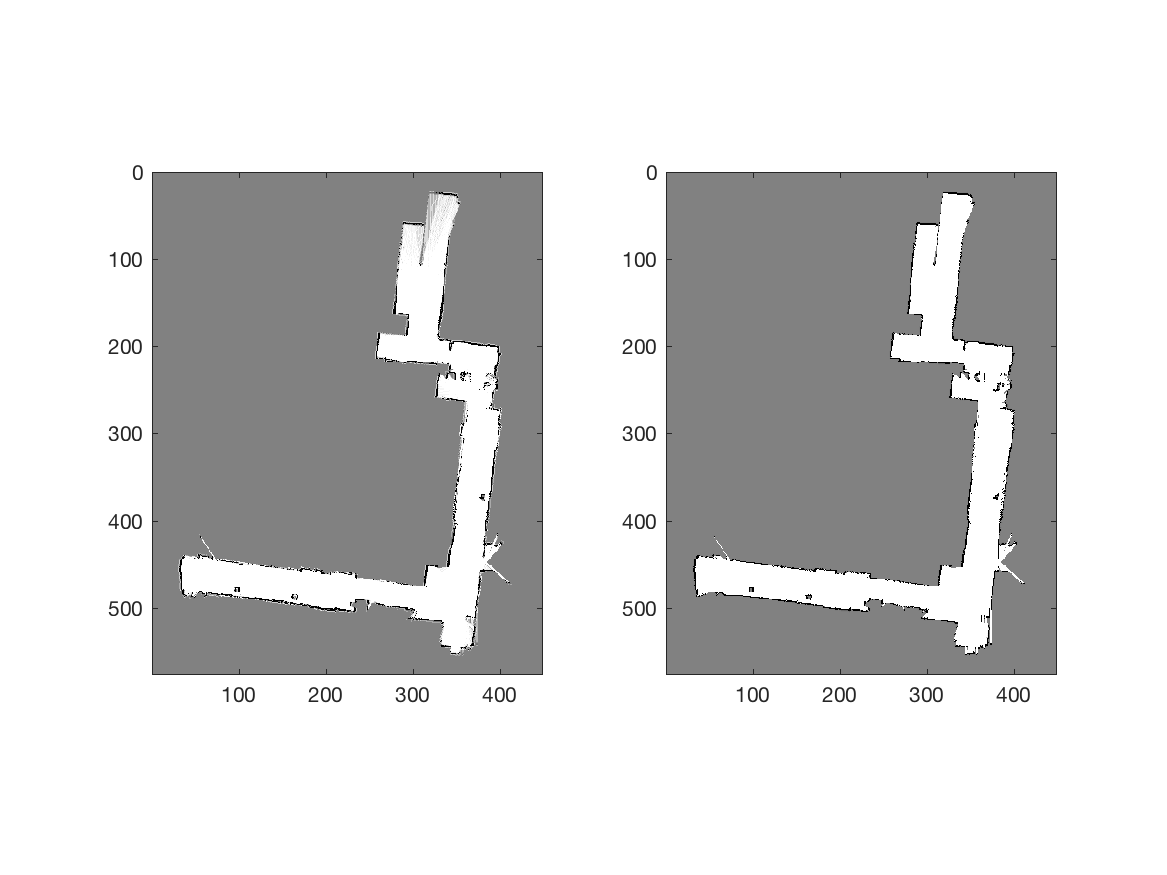
\includegraphics[trim={1.5cm 3.5cm 1.5cm 1.5cm},clip,width=\textwidth]{map_comparison.png}
        \caption{Comparison of the total mapped environment based on the approximate (left) and proposed (right) inverse sensor model.}
        \label{fig:penn_map_total}
    \end{subfigure}
    \begin{subfigure}[t]{0.8\columnwidth}
        \centering
        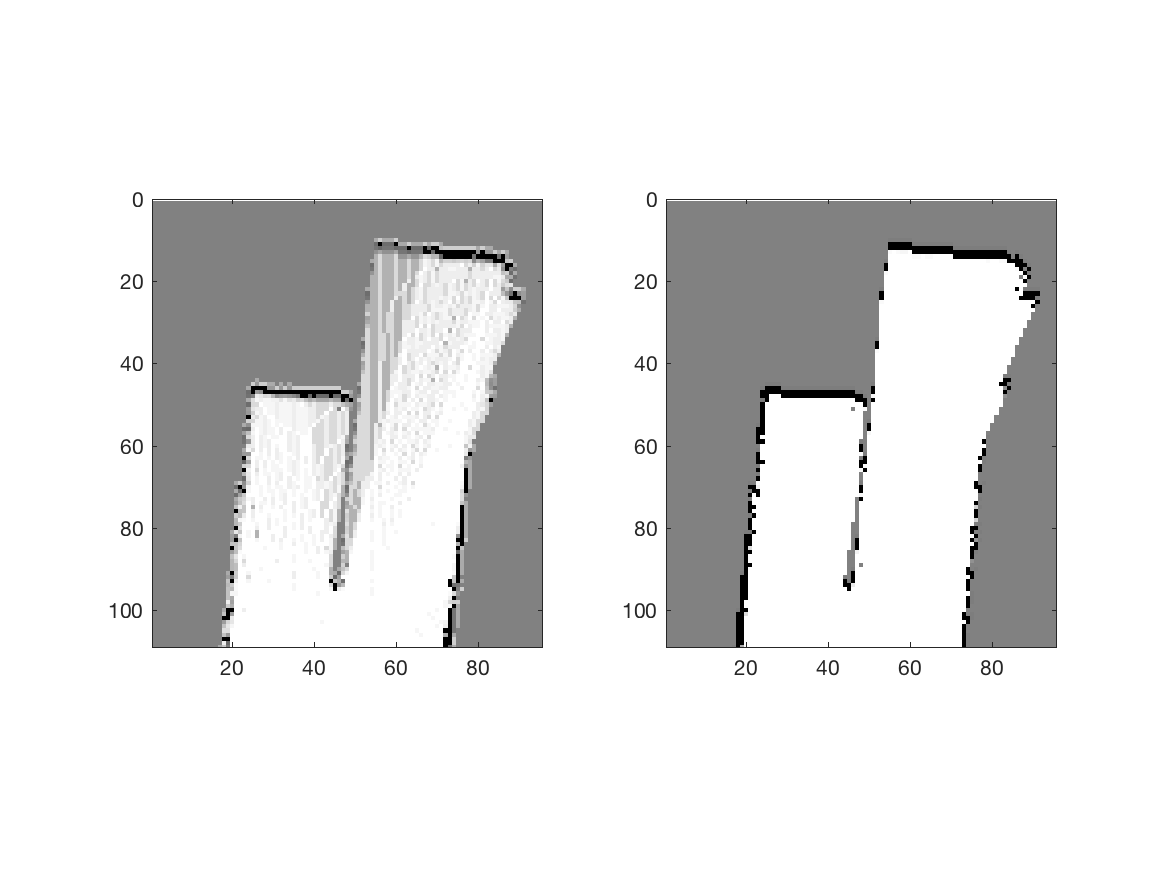
\includegraphics[trim={1.5cm 3.5cm 1.5cm 1.5cm},clip,width=\textwidth]{map_zoom.png}
        \caption{Evidence of significant improvement at certain area of the map.}
        \label{fig:penn_map_zoom}
    \end{subfigure}
    \caption{Comparison of Proposed Ray-By-Ray Approach with Approximate Solution}
	\medskip
	\small
	Using experimental sensor data, the map was generated using an approximate and the proposed exact inverse sensor models. The laser sensor and odometry data used for the experiment was provided by University of Pennsylvania open course robotics estimation and learning on Coursera~\cite{coursera}.
    \label{fig:penn_map}
\end{figure}


\begin{figure}[!ht]
    \centering
    \begin{subfigure}[t]{0.35\columnwidth}
        \centering
        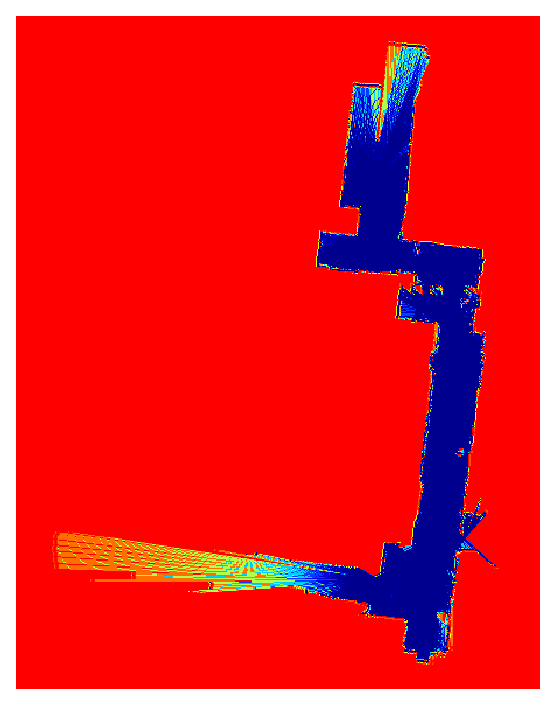
\includegraphics[width=\textwidth]{AISM_Image_inf_19.pdf}
        \caption{Approximate inverse sensor model}
        \label{fig:AISM}
    \end{subfigure}
    \begin{subfigure}[t]{0.35\columnwidth}
        \centering
        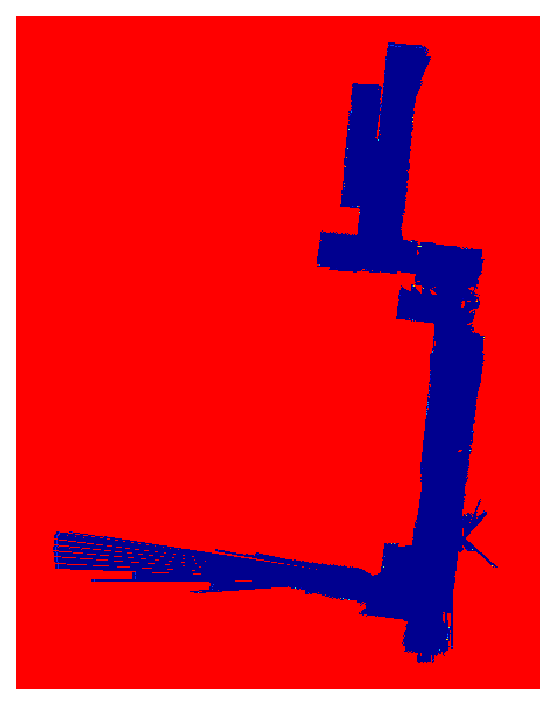
\includegraphics[width=\textwidth]{EISM_Image_inf_19.pdf}
        \caption{Exact inverse sensor model}
        \label{fig:EISM}
    \end{subfigure}
    \caption{Map Uncertainty Comparison Between Proposed Ray-By-Ray Approach and Approximate Solution}
	\medskip
	\small
	The entropy is compared between the approximate and proposed exact inverse sensor models at step 2280. The blue areas show the lowest entropy while red shows highest.
\label{fig:entropy_comp}
\end{figure}


\begin{figure}
  \centering
  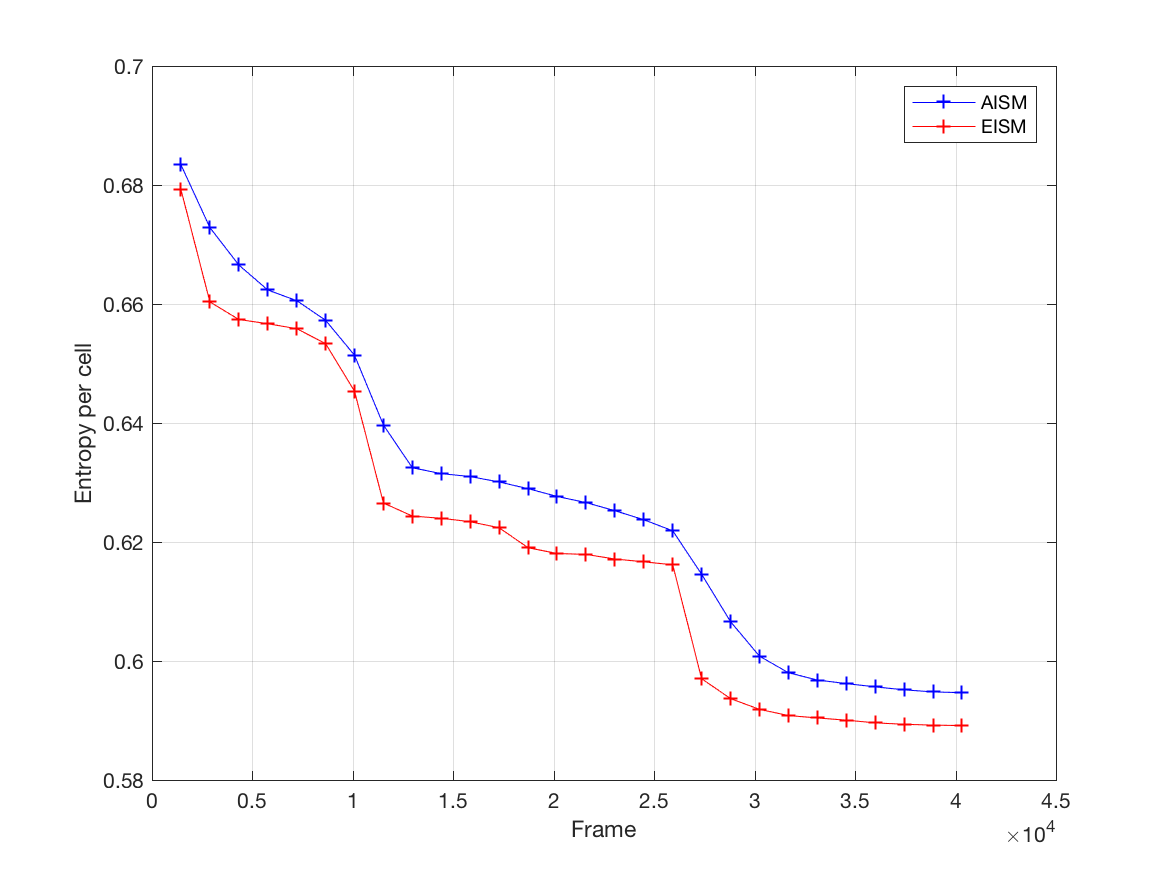
\includegraphics[width=0.7\textwidth]{entropy_frame.png}
  \caption{Entropy Histories of the Proposed Ray-By-Ray Approach and Approximate Solution}
  	\medskip
	\small
	The map entropies of the approximate inverse sensor model (blue) and the proposed exact inverse sensor model (red) show that the exact version yields a more certain occupancy grid map.
\label{fig:entropy}
\end{figure}



\paragraph{Mapping a Room with the Synergistic Approach}

Next, we compare the same approximate inverse sensor model against the synergistic exact inverse sensor model.
Here, the robot maps in a two-dimensional environment composed of ten wall edges, and the robot follows a figure-eight curve, then turns around and completes the same curve in the reverse direction. Like the prior example, the same set of measurements updated each second are used with both occupancy grid mapping algorithms to construct the map.
The resulting maps are illustrated in Figure \ref{fig:NumResOccProbs} for both algorithms, where it is shown that the proposed algorithm yields a substantially more accurate and clear map with less uncertainty. 

\begin{figure}
%    \centering{
%    \begin{subfigure}[t]{0.4\columnwidth}
%        \centering
%        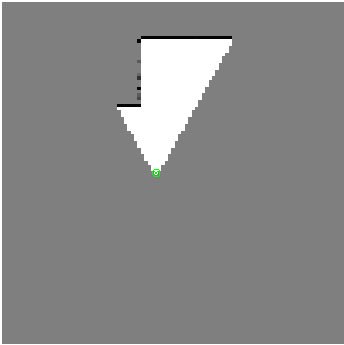
\includegraphics[width=0.7\columnwidth]{Compare_ISM_1.png}
%        \caption{Map at $t=0$ sec (exact)}
%    \end{subfigure}
%    \begin{subfigure}[t]{0.4\columnwidth}
%        \centering
%        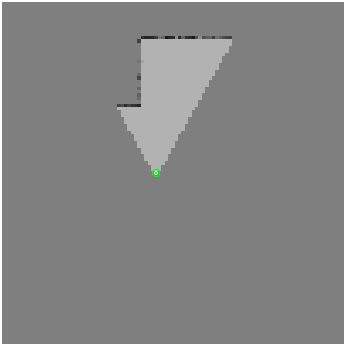
\includegraphics[width=0.7\columnwidth]{Compare_Approx_1.png}
%        \caption{Map at $t=0$ sec (approx.)}
%    \end{subfigure}
%    }
    \centering{
    \begin{subfigure}[t]{0.4\columnwidth}
        \centering
        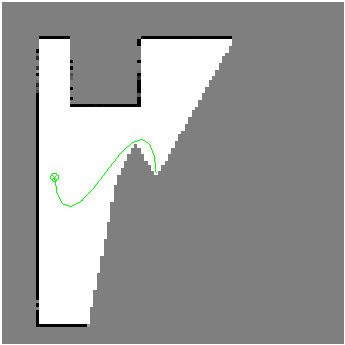
\includegraphics[width=0.7\columnwidth]{Compare_ISM_2.png}
        \caption{Map at $t=13$ sec (exact)}
    \end{subfigure}
    \hspace*{-0.05\columnwidth}
    \begin{subfigure}[t]{0.4\columnwidth}
        \centering
        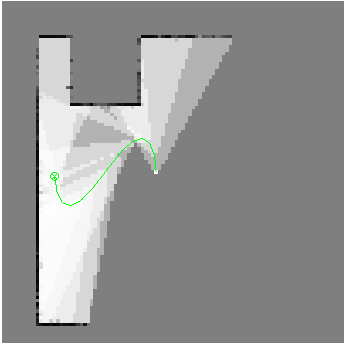
\includegraphics[width=0.7\columnwidth]{Compare_Approx_2.png}
        \caption{Map at $t=13$ sec (approx.)}
    \end{subfigure}
    }
    \centering{
    \begin{subfigure}[t]{0.4\columnwidth}
        \centering
        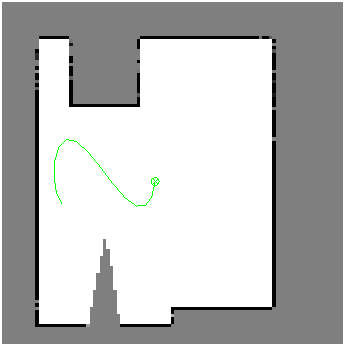
\includegraphics[width=0.7\columnwidth]{Compare_ISM_3.png}
        \caption{Map at $t=25$ sec (exact)}
    \end{subfigure}
    \hspace*{-0.05\columnwidth}
    \begin{subfigure}[t]{0.4\columnwidth}
        \centering
        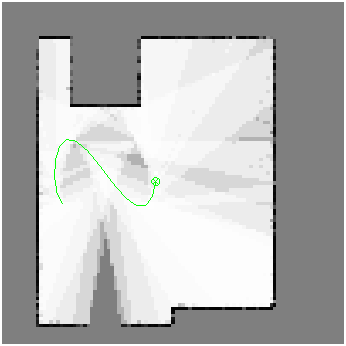
\includegraphics[width=0.7\columnwidth]{Compare_Approx_3.png}
        \caption{Map at $t=25$ sec (approx.)}
    \end{subfigure}
    }
    \centering{
    \begin{subfigure}[t]{0.4\columnwidth}
        \centering
        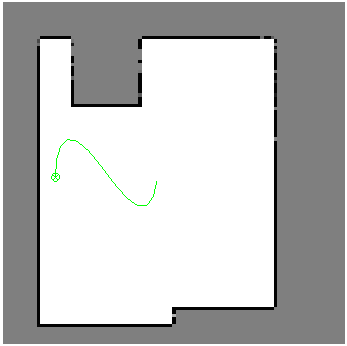
\includegraphics[width=0.7\columnwidth]{Compare_ISM_4.png}
        \caption{Map at $t=38$ sec (exact)}
    \end{subfigure}
    \hspace*{-0.05\columnwidth}
    \begin{subfigure}[t]{0.4\columnwidth}
        \centering
        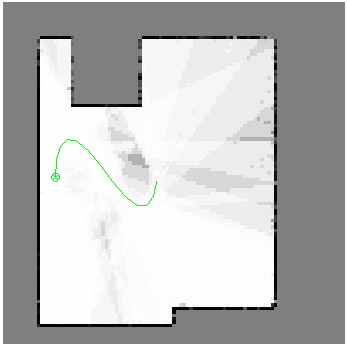
\includegraphics[width=0.7\columnwidth]{Compare_Approx_4.png}
        \caption{Map at $t=38$ sec (approx.)}
    \end{subfigure}
    }
    \centering{
    \begin{subfigure}[t]{0.4\columnwidth}
        \centering
        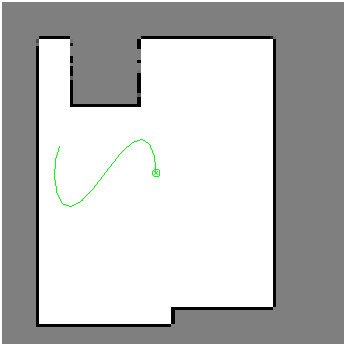
\includegraphics[width=0.7\columnwidth]{Compare_ISM_5.png}
        \caption{Map at $t=50$ sec (exact)}
    \end{subfigure}
    \hspace*{-0.05\columnwidth}
    \begin{subfigure}[t]{0.4\columnwidth}
        \centering
        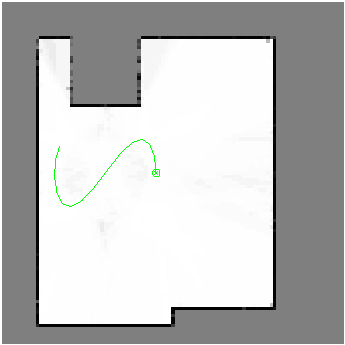
\includegraphics[width=0.7\columnwidth]{Compare_Approx_5.png}
        \caption{Map at $t=50$ sec (approx.)}
    \end{subfigure}
    }
    \caption{Comparison of Proposed Synergistic Approach with Approximate Solution}
	\medskip
	\small
	A robot (green crossed circle, green curve of its previous $13$ seconds) measures a room with a Kinect depth sensor. Grid cells are either known as free (white) or occupied (black), or uncertain (gray).
\label{fig:NumResOccProbs}
\end{figure}


The change of the map entropy over time, and the entropy of the completed maps, for both methods are depicted in Figure \ref{fig:NumResOccH}. The subfigure \ref{fig:NumResOccHa} illustrates that the proposed exact inverse sensor model exhibits rapid decreases of entropies, and smaller entropies always. The resulting terminal map obtained from the proposed approach, shown in the subfigure \ref{fig:NumResOccHb}, has less uncertainty than \ref{fig:NumResOccHc} constructed by the approximate model. In short, the proposed approach is more efficient at extracting information about the environment from the same set of set measurements. 


\begin{figure}
    \centering{
    \begin{subfigure}[t]{0.8\columnwidth}
        \centering
        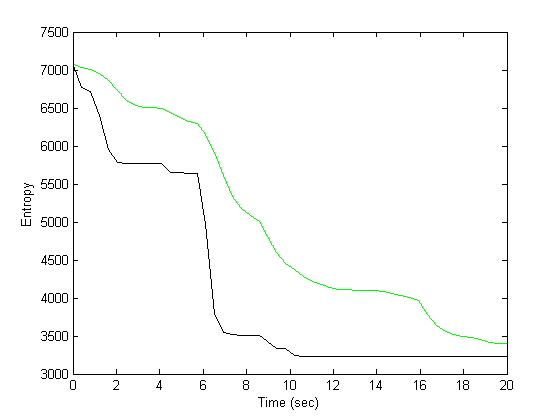
\includegraphics[width=0.7\columnwidth]{EntropyEvolution.png}
        \caption{Entropy (black: exact model, green: approx.)}
        \label{fig:NumResOccHa}
    \end{subfigure}
}
    \centering{
    \begin{subfigure}[t]{0.4\columnwidth}
        \centering
        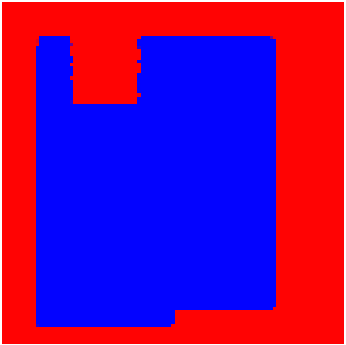
\includegraphics[width=0.7\columnwidth]{Compare_ISM_H.png}
        \caption{Entropy map at $t=50$ (exact)}
        \label{fig:NumResOccHb}
    \end{subfigure}
    \begin{subfigure}[t]{0.4\columnwidth}
        \centering
        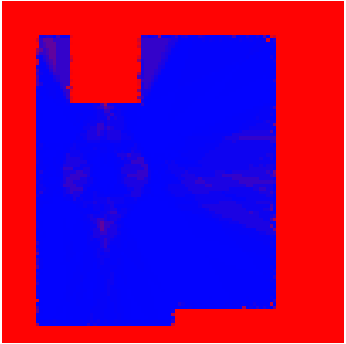
\includegraphics[width=0.7\columnwidth]{Compare_Approx_H.png}
        \caption{Entropy map at $t=50$  (approx.)}
        \label{fig:NumResOccHc}
    \end{subfigure}
    }
    \caption{Map Uncertainty Comparison Between Proposed Synergistic Approach and Approximate Solution}
	\medskip
	\small
	Entropy serves as a measure of uncertainty of the occupancy grid, where more blue regions are more certain, and red regions are more uncertain. The uncertainty is always less when the exact solution is applied.
\label{fig:NumResOccH}
\end{figure}


% I think I'll skip this trivial result:
%\subsection{Kinect Measurement Scan Analysis}
%% ACC16 Single scan exact/approx. comparison




\section{Conclusions}

In this chapter, we presented the exact solution to the inverse sensor model for a single measurement ray, then extended this result to 2D occupancy grids. Measurement scans were analyzed with two techniques, namely ray-by-ray and synergistic combinations. Then, numerical results show how both proposed solutions outperform existing approximate solutions. Upon further study, the ray-by-ray approach has proven more robust against localization errors and changing environments because the rays are not assumed completely independent. Therefore, the ray-by-ray approach is applied to the subsequent proposals, numerical simulations, and experimental results.





